\begin{center}
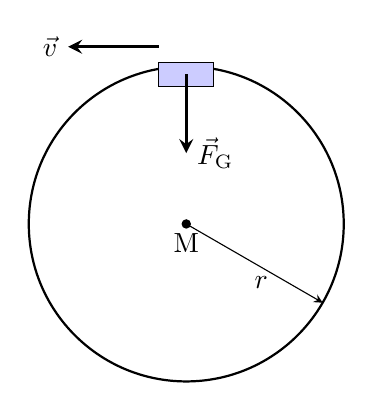
\begin{tikzpicture}[>=stealth]
 \draw[thick] (0,0) circle (2);
 \fill (0,0) circle (0.06) node[below] {M};
 \draw[->] (0,0) -- (-30:2) node[pos=0.55, below] {$r$};
 \fill[blue!20] (-0.35,1.75) rectangle (0.35,2.05);
 \draw (-0.35,1.75) rectangle (0.35,2.05);
 \draw[->, very thick] (0,1.9) -- (0,0.9) node[right] {$\vec F_\mathrm{G}$};
 \draw[->, very thick] (-0.35,2.25) -- (-1.5,2.25) node[left] {$\vec v$};
\end{tikzpicture}
\end{center}

Im höchsten Punkt zeigen die Gewichtskraft und die Normalkraft der Bahn beide nach unten, zum Mittelpunkt. Zusammen bilden sie die Zentripetalkraft:
\begin{align}
 F_\mathrm{G} + F_\mathrm{N} &= \frac{m\,v^2}{r}
\end{align}
Am langsamsten ist der Körper, wenn die Bahn gerade keine Kraft mehr ausübt ($F_\mathrm{N} = 0$) und die Gewichtskraft allein die Zentripetalkraft liefert: $m\,g = \frac{m\,v^2}{r}$. Damit
\begin{align}
 v_\mathrm{min} &= \vLoF = \sqrt{\gE\cdot\rLo} = \vLo \approx \result{\vLoP{0}{2}}
\end{align}
Ist der Körper schneller, reicht die Gewichtskraft nicht aus: Die Bahn muss zusätzlich mit einer Normalkraft nach unten drücken, der Körper wird an die Bahn gepresst. Ist er langsamer, ist die Gewichtskraft grösser als die nötige Zentripetalkraft: Der Körper löst sich von der Bahn und fällt auf einer Wurfparabel nach innen (sofern er nicht durch Schienen oder Gurte gehalten wird).
